\section*{\hfill{}УСЛОВИЕ\hfill{}}
В информационный центр приходят клиенты через интервал времени 10 $\pm$ 2 минуты. Если все три имеющихся оператора заняты, клиенту отказывают в обслуживании. Операторы имеют разную производительность и могут обеспечивать обслуживание среднего запроса пользователя за 20 $\pm$ 5; 40 $\pm$ 10; 40 $\pm$ 20. Клиенты стремятся занять свободного оператора с максимальной производительностью. Полученные запросы сдаются в накопитель. Откуда выбираются на обработку. На первый компьютер запросы от 1 и 2-ого операторов, на второй – запросы от 3-его. Время обработки запросов первым и 2-м компьютером равны соответственно 15 и 30 мин. Промоделировать процесс обработки 300 запросов. Определить вероятность отказа.

\section*{\hspace{1.25cm}1\quad{}Теоретическая часть}
На рисунке\ref{img:concept} изображена структурная схема рассматриваемой концептуальной модели.
\begin{figure}[H]
    \centering
    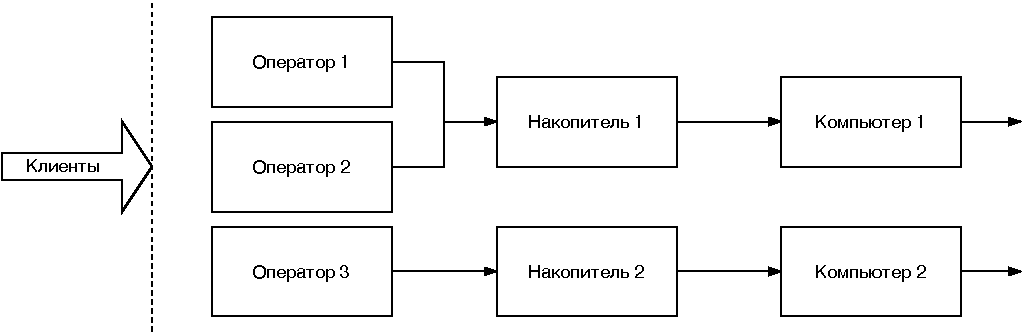
\includegraphics[width=0.8\textwidth]{pdf/concept.pdf}
    \caption{Структурная схема}
    \label{img:concept}
\end{figure}

\section*{\hspace{1.25cm}2\quad{}Результаты}
Вероятность отказа~--- это промежуток, поэтому прогоним модель 10 раз и выберем минимальное и максимальное значения.

На рисунке~\ref{img:results} представлены результаты выполнения программы.
\begin{figure}[H]
    \centering
    
\includegraphics[width=0.6\textwidth]{images/scr01.png}
    \caption{Результаты}
    \label{img:results}
\end{figure}

\section*{\hfill{}ВЫВОД\hfill{}}
В настоящей лабораторной работе была промоделирована информационная система, в которую поступают клиенты. Эта система состоит нескольких блоков, а именно: генератор заявок, три оператора, два накопителя и два компьютера. Выходными данными являются вероятность отказа и количество клиентов, отказ получивших.
